\documentclass[aspectratio=43]{beamer}
\mode<presentation>
\usetheme{Madrid}
\usecolortheme{seahorse}
% \usepackage[table]{xcolor}
\usepackage{multimedia}
\usepackage{media9}
\usepackage[utf8]{inputenc}
\usepackage{amsmath}
\usepackage{lmodern}
% \usepackage[usenames, dvipsnames]{color}

\usepackage{arydshln}
\usepackage{url}
\usepackage[absolute,overlay]{textpos}
% \usepackage[texcoord,grid,gridunit=cm,gridcolor=red!50,subgridcolor=green!50]{eso-pic}
\setlength{\TPHorizModule}{\textwidth}
\setlength{\TPVertModule}{\textwidth}

\graphicspath{{plots/}}

\setbeamercolor{CBwonb}{fg=white,bg=white!10!blue}
\setbeamercolor{CBronb}{fg=red,bg=white!10!blue}

\usepackage{tikz}
\usetikzlibrary{shapes,arrows,positioning}
\tikzstyle{startstop} = [rectangle, rounded corners, minimum width=1cm, minimum height=0.1cm,text centered, text width=2.5cm, draw=black, fill=red!30]
\tikzstyle{io} = [trapezium, trapezium left angle=70, trapezium right angle=110, minimum width=1cm, minimum height=0.1cm, text centered, text width=2.5cm, draw=black, fill=blue!30]
\tikzstyle{process} = [rectangle, minimum width=1cm, minimum height=0.1cm, text centered,text width=2.5cm, draw=black, fill=orange!30]
\tikzstyle{decision} = [circle, minimum width=1cm, minimum height=0.1cm, text centered,text width=2.5cm, draw=black, fill=green!30]
\tikzstyle{arrow} = [thick,->,text centered, color=blue, text width=2cm,>=stealth]

\newcommand{\Msun}{~{\rm M_\sun}}
\newcommand{\hMsun}{~h^{-1}\>{\rm M_\odot}}
\newcommand{\Mpc}{~h^{-1}~{\rm Mpc}}
\newcommand{\Kpc}{~h^{-1}~{\rm kpc}}


\title[]{The Large-Scale Environments}
\subtitle{The large-scale distribution of baryons inside the cosmological
hydrodynamical simualtions.}
\author[Email: weiguang.cui@uam.es]{{\Large \bf Weiguang Cui},
\inst{*} \footnote{\url{https://weiguangcui.github.io}}}
\institute[]{
  \inst{*}
  Departamento de F\'isica Te\'{o}rica, \\
  Universidad Aut\'{o}noma de Madrid, 28049 Madrid, Spain
}
\date[]{The HUBS workshop, @ Shanghai. \\  October, 16, 2018}
\logo{
\includegraphics[height=1cm]{logo_uam.jpg}}

%%%%%%%%%%%%%%%%%%%%%%%%%%%%%%%%%%%%%%%%%%%%%%%%%%%%%%%%%%%%%%%%%%%%%%%%%
\begin{document}
  \frame{\titlepage}

%----------------------------------
\section{Introduction} \label{sec:1}

\begin{frame}{Background:}
The content of the Universe:
\begin{figure}
    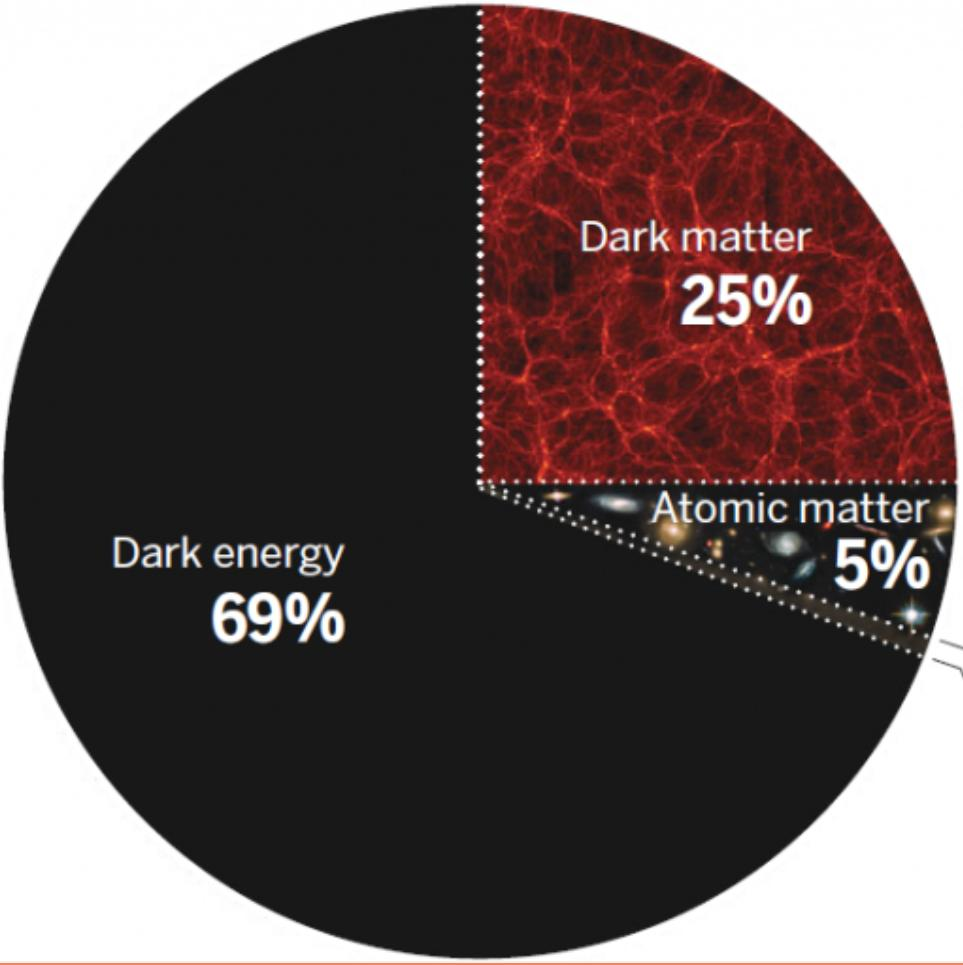
\includegraphics[width=0.6\textwidth]{fraction.jpg}
\end{figure}
\begin{textblock*}{3cm}(9.8cm,6.6cm)
{$\sim$1\% of neutrinos, etc.}
\end{textblock*}
\end{frame}

\begin{frame}
  \frametitle{Background: the distribution of dark matter at large scale}
  \framezoom<1><2>[](5cm,3.5cm)(1.5cm,1.5cm)
  \begin{figure}
    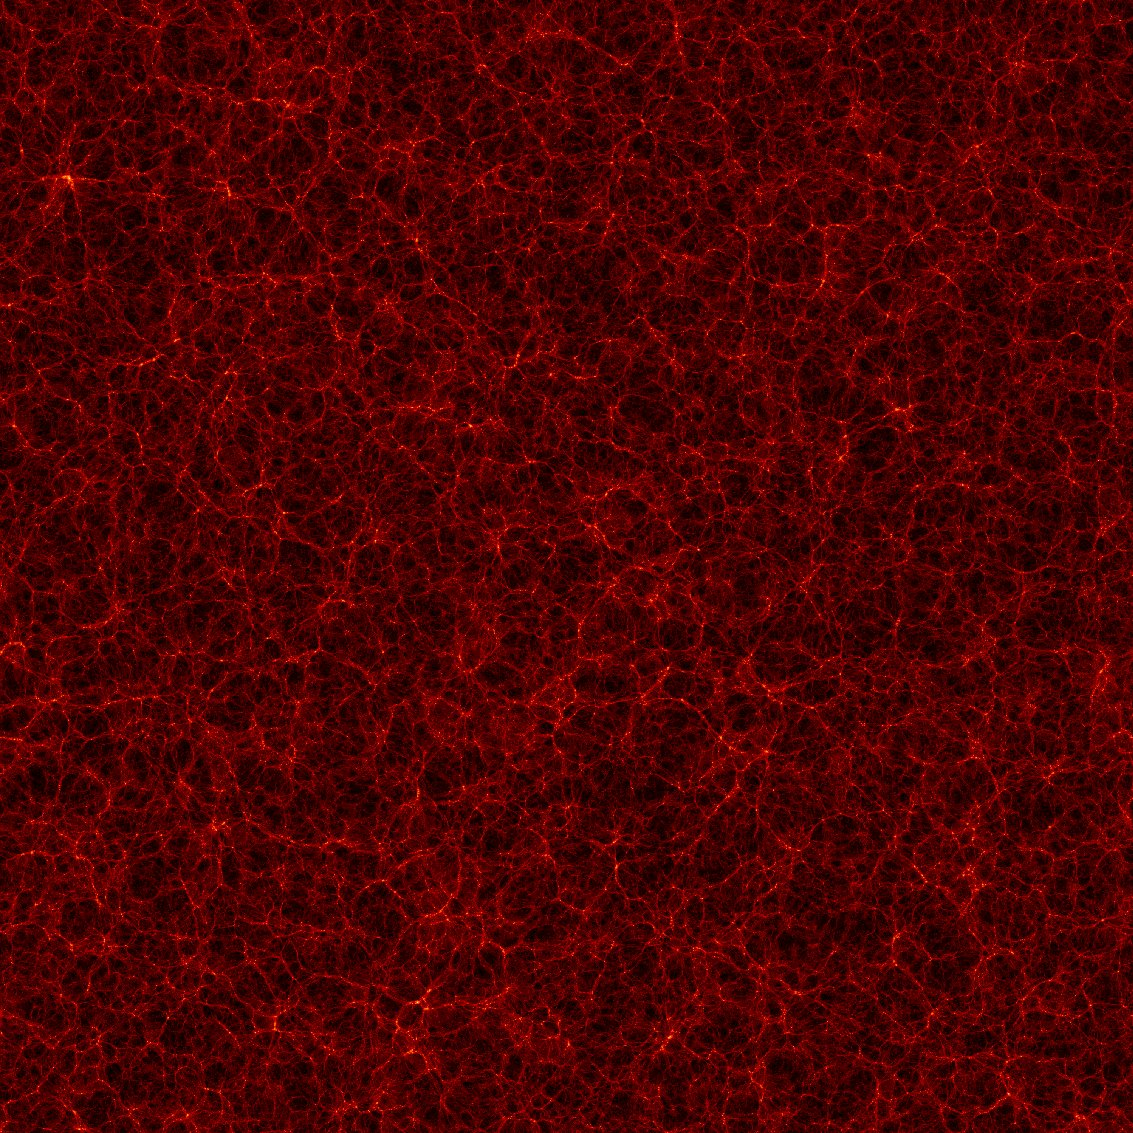
\includegraphics[width=0.6\textwidth]{mdpl.jpg}
  \end{figure}
  \begin{textblock*}{2.5cm}(10.2cm,6cm)
    {Credit: MultiDark Planck simulation}
  \end{textblock*}
\end{frame}

\begin{frame}{Background:}
The content of the Universe:
\begin{figure}
    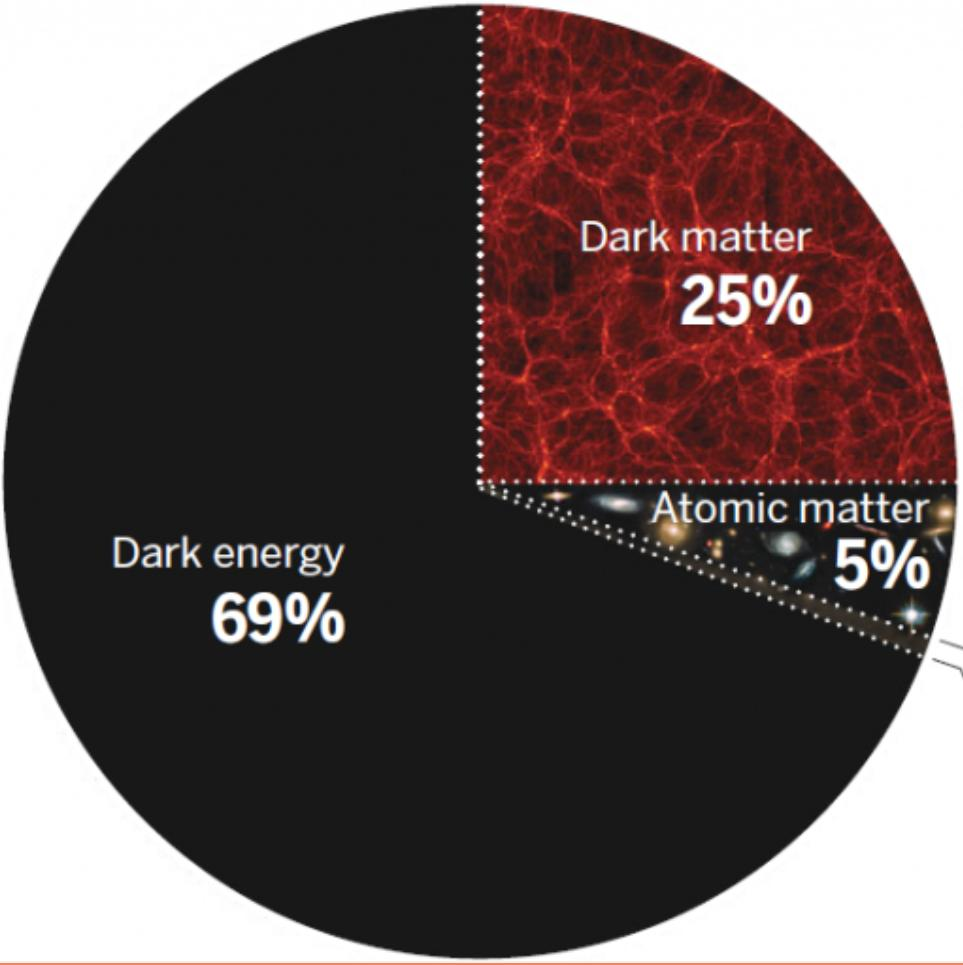
\includegraphics[width=0.6\textwidth]{fraction.jpg}
\end{figure}
\begin{textblock*}{3cm}(9.8cm,6.6cm)
{$\sim$1\% of neutrinos, etc.}
\end{textblock*}
\end{frame}

\begin{frame}
  \frametitle{Background: the distribution of galaxies at large-scale}
  \framezoom<1><2>(2.cm,2.5cm)(2.cm,2.cm)
  \begin{figure}
    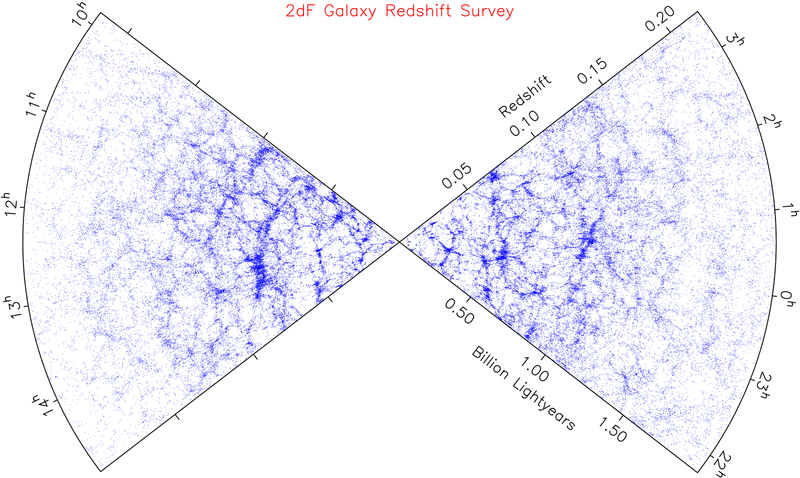
\includegraphics[width=0.9\textwidth]{2dFzcone.jpg}
  \end{figure}
  \begin{textblock*}{4cm}(5cm,8.5cm)
    {Credit: Yang et al. 2005}
  \end{textblock*}
\end{frame}

\begin{frame}{Background: the fractions}
The content of the Universe:
  \begin{figure}
    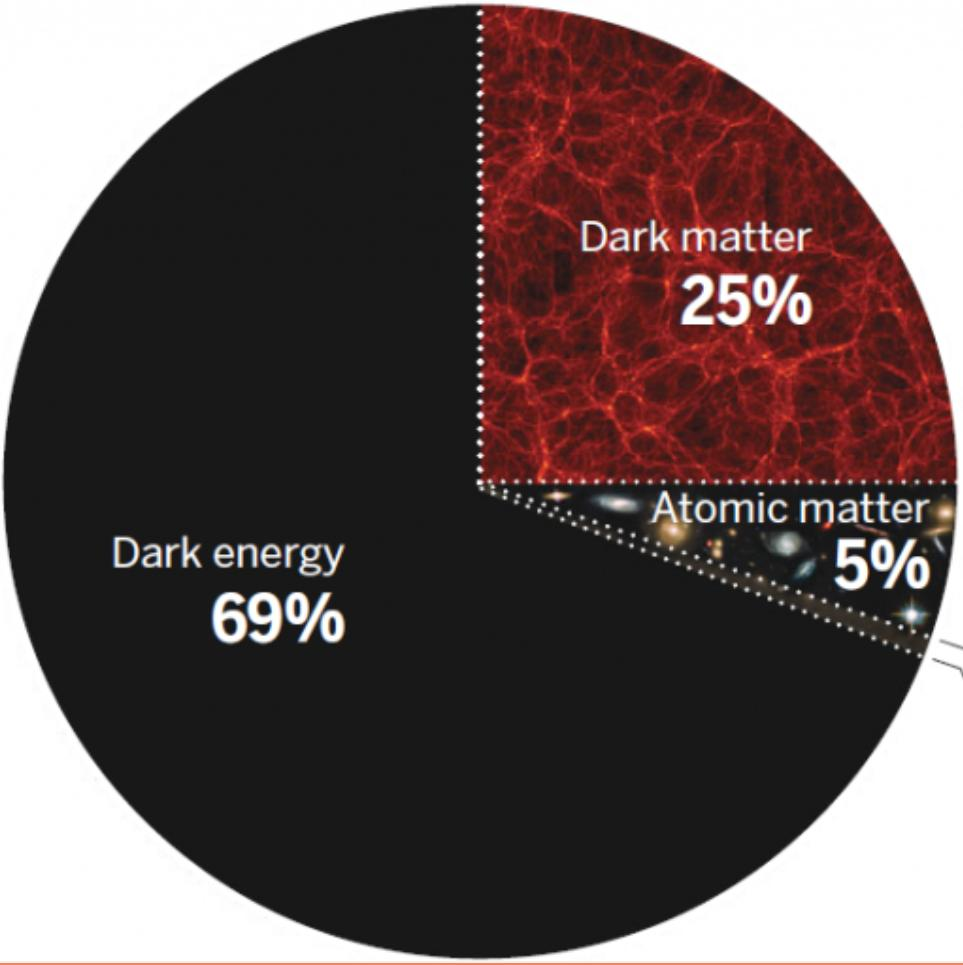
\includegraphics[width=0.6\textwidth]{fraction.jpg}
  \end{figure}
  \begin{textblock*}{3cm}(9.8cm,6.6cm)
    {$\sim$1\% of neutrinos, etc.}
  \end{textblock*}
  \begin{textblock*}{2.6cm}(10.cm,5.2cm)
    {\color{red}{Stars only account for $\sim$0.07\%}}
  \end{textblock*}
\end{frame}

\begin{frame}{Background: waht and where is the others??}
  \begin{figure}
    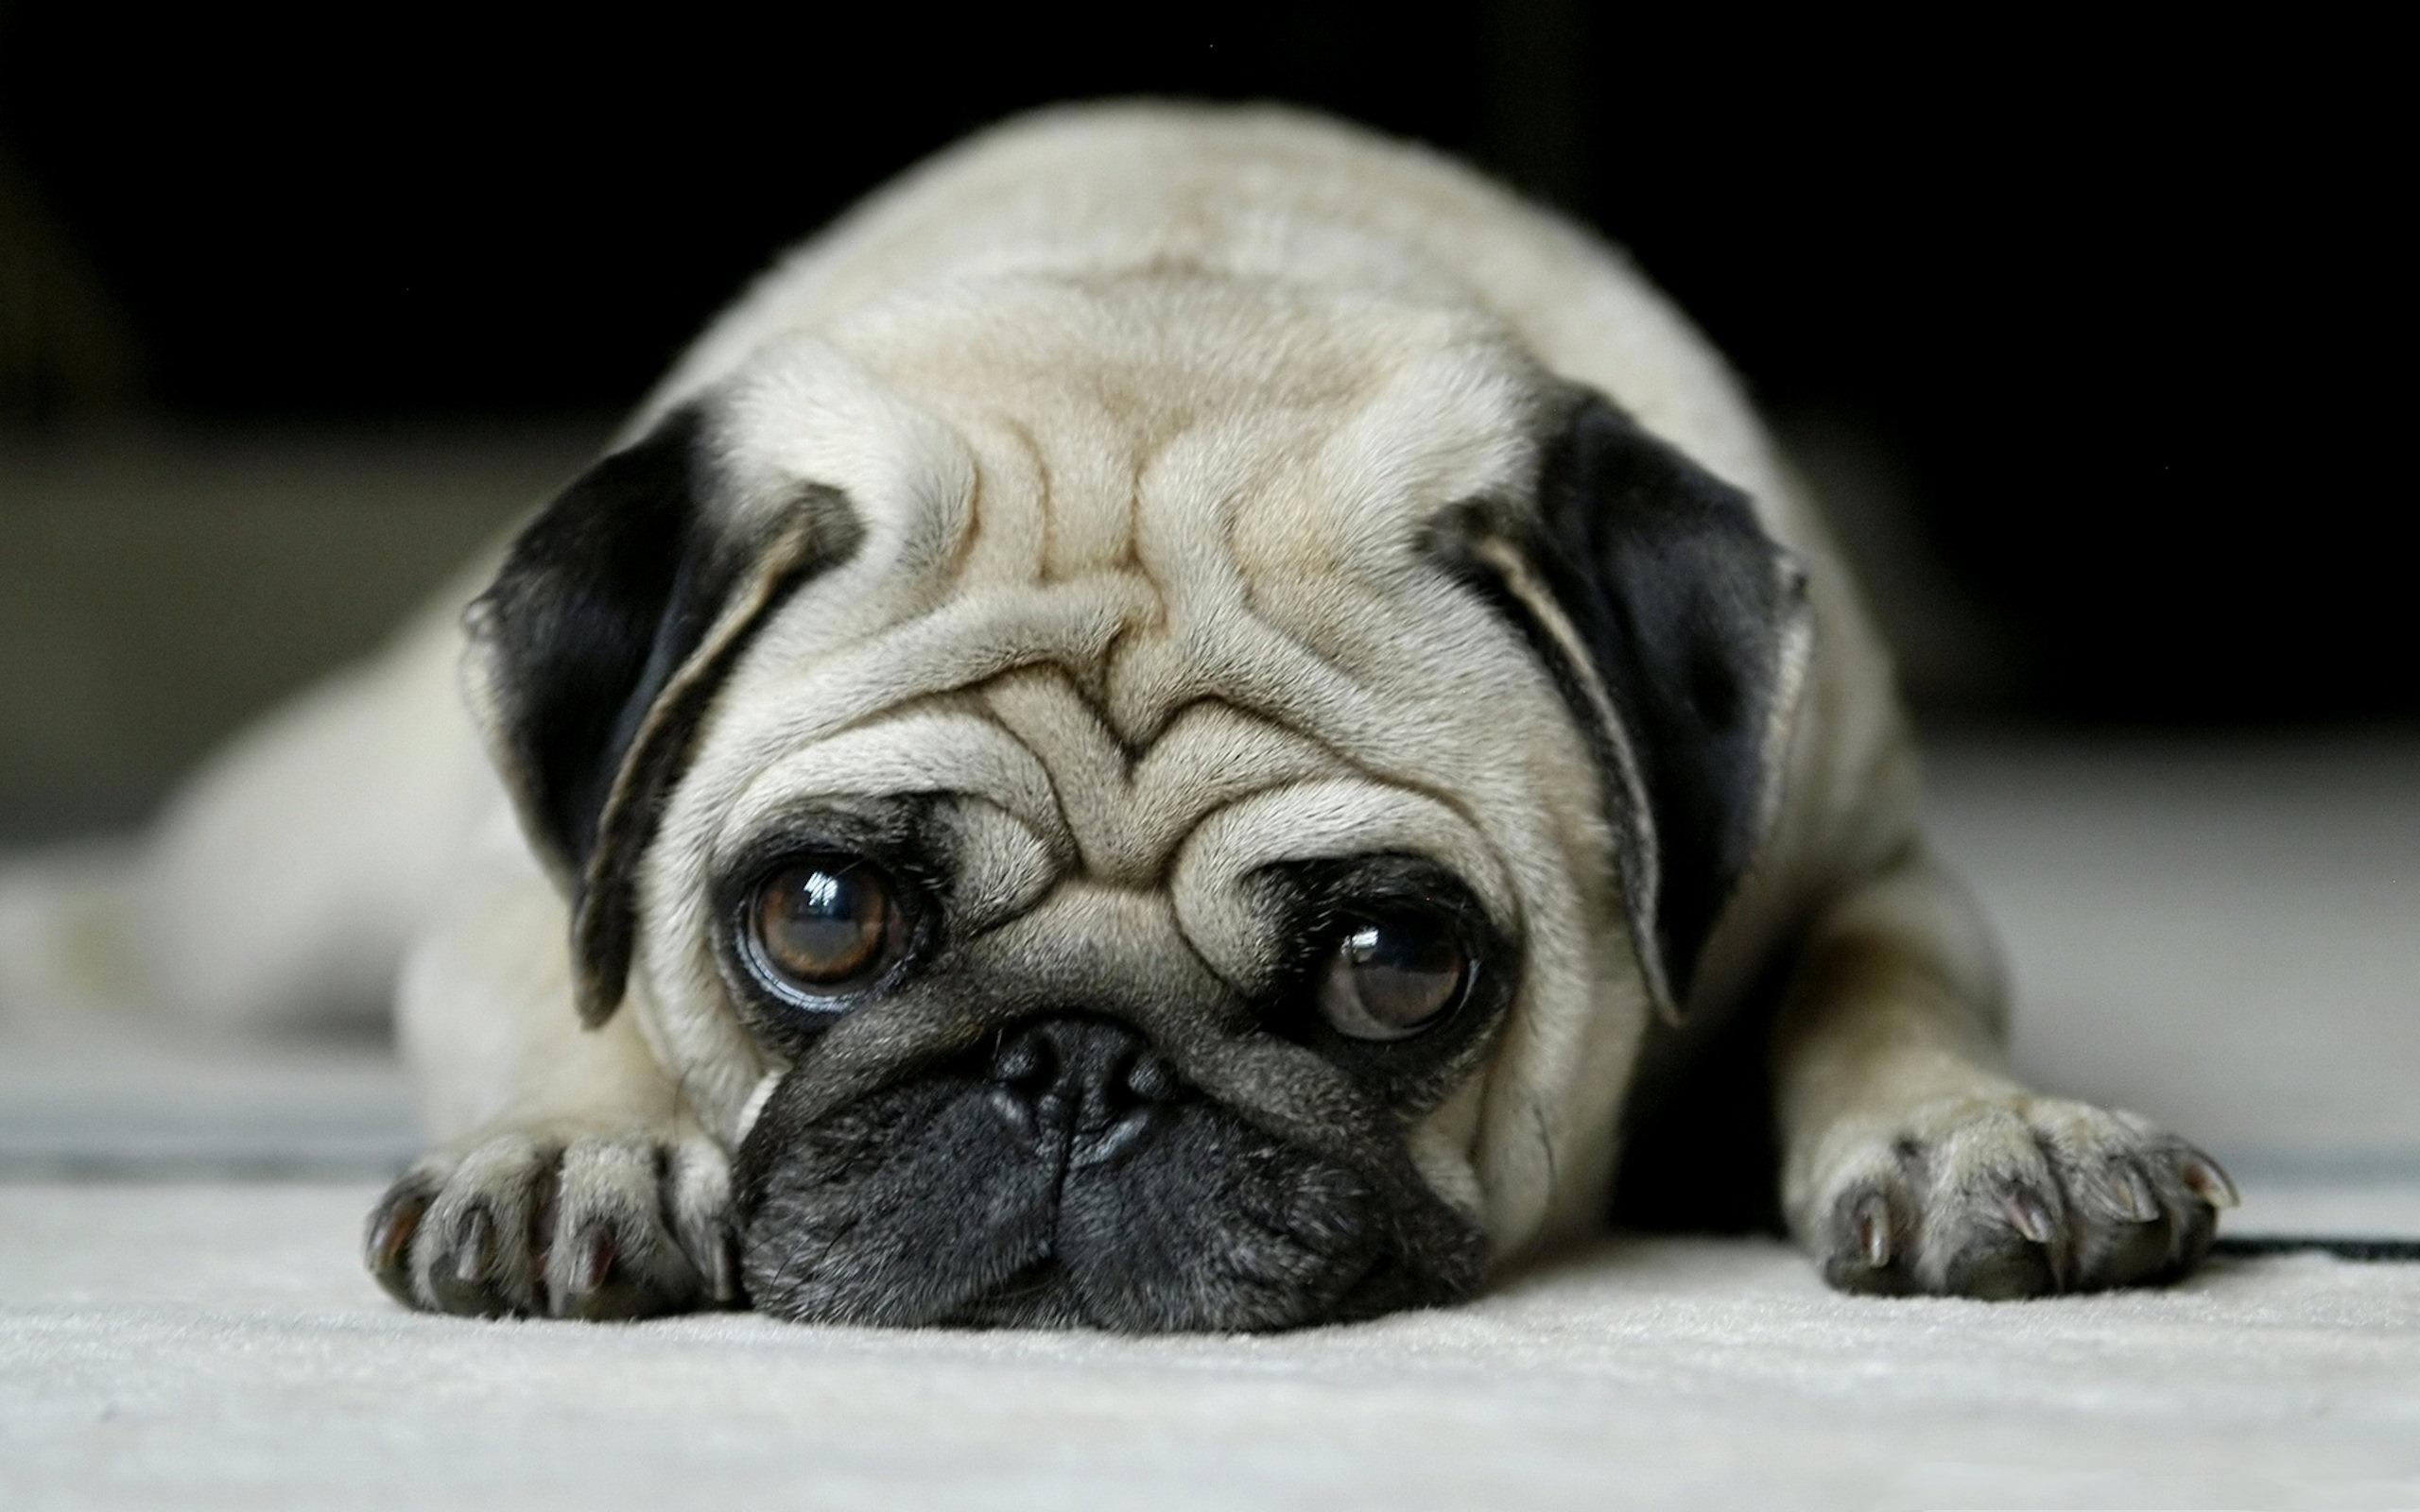
\includegraphics[width=\textwidth]{lonely-dog.jpg}
  \end{figure}
  \only<2-3>{
    \begin{textblock*}{15cm}(2cm,2.5cm)
      {\huge \color{green}{Cold gas + Hot gas + WHIM}}
    \end{textblock*}  
    }
  \only<3>{
    \begin{textblock*}{15cm}(2.5cm,4cm)
      {\Huge \color{red}{WHIM: WHy I'M here?}}
    \end{textblock*}
  }
\end{frame}

\begin{frame}
  \frametitle{What is in this talk?}
  To study the distribution and abundance of baryonic matter at large-scale environments.
  \begin{itemize}
    \item<1-> The hydro-simulations for this study.
    \item<2-> How to classify the large-scale environments?
    \item<3-> What does the simulation say about the baryon distribution?
    \item<4-> Conclusion and future prospects.
  \end{itemize}
  % \only<1>{
  %   \begin{center}
  %     {\Large \bf The {\sc nIFTy} galaxy cluster comparison project}\footnote{\scriptsize Ref: Sembolini et al. 2016a,b; Elahi et al. 2016; Cui et al. 2016; Arthur et al. 2017}
  %   \end{center}
  %   \alert{11} different (in both algorithms and baryon models) simulation codes are used to simulate the same galaxy cluster.
  % }
  % \only<2>{
  %   \begin{center}
  %     {\Large \bf What did we find? I}
  %   \end{center}
  %   {\scriptsize
  %   \begin{itemize}
  %     \item The modern SPH codes produce correct entropy profiles as AMR, moving mesh.
  %     \item The baryon models have larger effects than the fluid simulating techniques by mixing the entropy profiles.
  %   \end{itemize}}
    % \begin{figure}
    %   \vspace{-0.2cm}
    %   \includegraphics<2>[width=0.36\textwidth]{nifty-entropy.png}
    %   \includegraphics<2>[width=0.45\textwidth]{nifty-entropy-fp.png}\vspace{-0.4cm}
    %   % \caption{{\scriptsize Entropy profile. Ref: Sembolini et al. 2016a,b}}
    % \end{figure}
    % \begin{textblock}{0.12}(0.01,0.3)
    %   {\scriptsize  Entropy profile. \\ Ref: Sembolini et al. 2016a,b.}
    % \end{textblock}
  % }
\end{frame}

\section{simulations}
\begin{frame}{The cosmological hydrodynamical simulations}
Three versions of simulations with different sets of baryonic models are used for this study:
\begin{itemize}
    \item RDM -- dark-matter-only simulation; 
    \item CSF -- gas Cooling, Star formation and Supernovae feedback;
    \item AGN -- additional BH evolution and feedback are also included.
\end{itemize}
\vspace{-0.6cm}
\begin{table}
\fontsize{9}{9}\selectfont
\caption{Parameters of the Three Hundred simulations}
\begin{tabular}{lll}
  \hline
  Parameter& Value & Description\\
  \hline
  $\Omega_M$ & 0.24 & Total Matter density parameter\\
  $\Omega_B$ & 0.041 & Baryon density parameter\\
  $\Omega_\Lambda$ & 0.76 & Cosmological Constant density parameter\\
  $h$ & 0.73  & Hubble constant in units of 100 km/s/Mpc\\
  $\sigma_8$ & 0.8 & Normalization of Power spectrum\\
  $n_s$ & 0.96  & Power index\\
  $\epsilon_{phys}$ & 7.5 & Plummer equivalent softening in $\Kpc$ \\
  Box size & \alert{410} & [$\Mpc$] The simulation box size on one side \\
  Particle mass & $7.6 (35.4) $ & [$10^8 \hMsun$] gas (DM) particle mass \\
  \hline
\end{tabular}
\end{table}
Details can be found in Cui et al. 2014.
\end{frame}

\begin{frame}{The overall baryon fractions}
    Following Dave et al. 2001, gas is separated into:
    \begin{itemize}
        \item[] Hot gas: T $>$ 10$^7$ K 
        \item[] WHIM: 10$^5 >$ T $> 10^7$ K 
    \end{itemize}
    
    \begin{table}[]
        \centering
        \begin{tabular}{c|c|c|c|}
            & $f_{hot gas}$ & $f_{WHIM}$ & $f_{star}$ \\
            \hline
           Nicastro et al. 2018 (z $<$ 0.5)  & $\sim$5\% & $\sim$24 -55 \% & $\sim$7 \% \\
           CSF (z = 0) & 4.6\% & 38.3\% & 6.5\% \\
           AGN (z = 0) & 4.6\% & 41.3\% & 3.2\% \\
           \hline
           CSF (z = 0.6) & 1.1\% & 29.7\% & 4.2\% \\
           AGN (z = 0.6) & 2.4\% & 34.9\% & 2.5\% \\
        \end{tabular}
        \caption{The mass fractions are with respect to the cosmic baryon fraction.}
        \label{tab:my_label}
    \end{table}
\end{frame}

\section{The classification methods}
\begin{frame}{The classification methods -- Vweb and Pweb\footnote{{\footnotesize Also called T-web}}}
\only<1->{
The re-scaled Poisson equation: $\Delta^2 \phi = \delta$ with $\delta$ the dimensionless matter overdensity and $\phi$ is the potential.}
\only<2->{
\vspace{-0.6cm}
  \begin{columns}[t]
    \begin{column}{0.49\textwidth}
      \begin{block}{Pweb:}
      The tidal tensor, $T_{\alpha\beta}$, is defined by the Hessian of the
gravitational potential $\phi$:
     $T_{\alpha\beta} = \frac{\partial^2\phi}{\partial r_{\alpha} \partial r_{\beta}}.$
      \end{block}
    \end{column}
    \begin{column}{0.49\textwidth}
      \begin{block}{Tweb :}
    The shear tensor, which is rewritten as
    $\Sigma_{\alpha, \beta} = -\frac{1}{2}(\frac{\partial v_{\alpha}}{\partial r_{\beta}} + \frac{\partial v_{\beta}}{\partial r_{\alpha}})/H_0$ 
      \end{block}
    \end{column}
  \end{columns}}
\only<3->{
 The three eigenvalues $\lambda_1 > \lambda_2 > \lambda_3$ are used to determine the large-scale environments:
 \begin{itemize}
     \item Voids: if $\lambda_1 < \lambda_{th}$
     \item Sheets: if $\lambda_1 >= \lambda_{th} > \lambda_2$
     \item Filaments: if $\lambda_2 >= \lambda_{th} > \lambda_3$
     \item Knots: $\lambda_3 >= \lambda_{th}$
 \end{itemize}}
\begin{textblock*}{3cm}(9.5cm,6cm)
{$\lambda_{th} = 0.01$ for Pweb; $\lambda_{th} = 0.1$ for Vweb}
\end{textblock*}
\end{frame}

\section{Results}
\begin{frame}{An illustration at z = 0}
\vspace{-0.3cm}
  \begin{figure}
    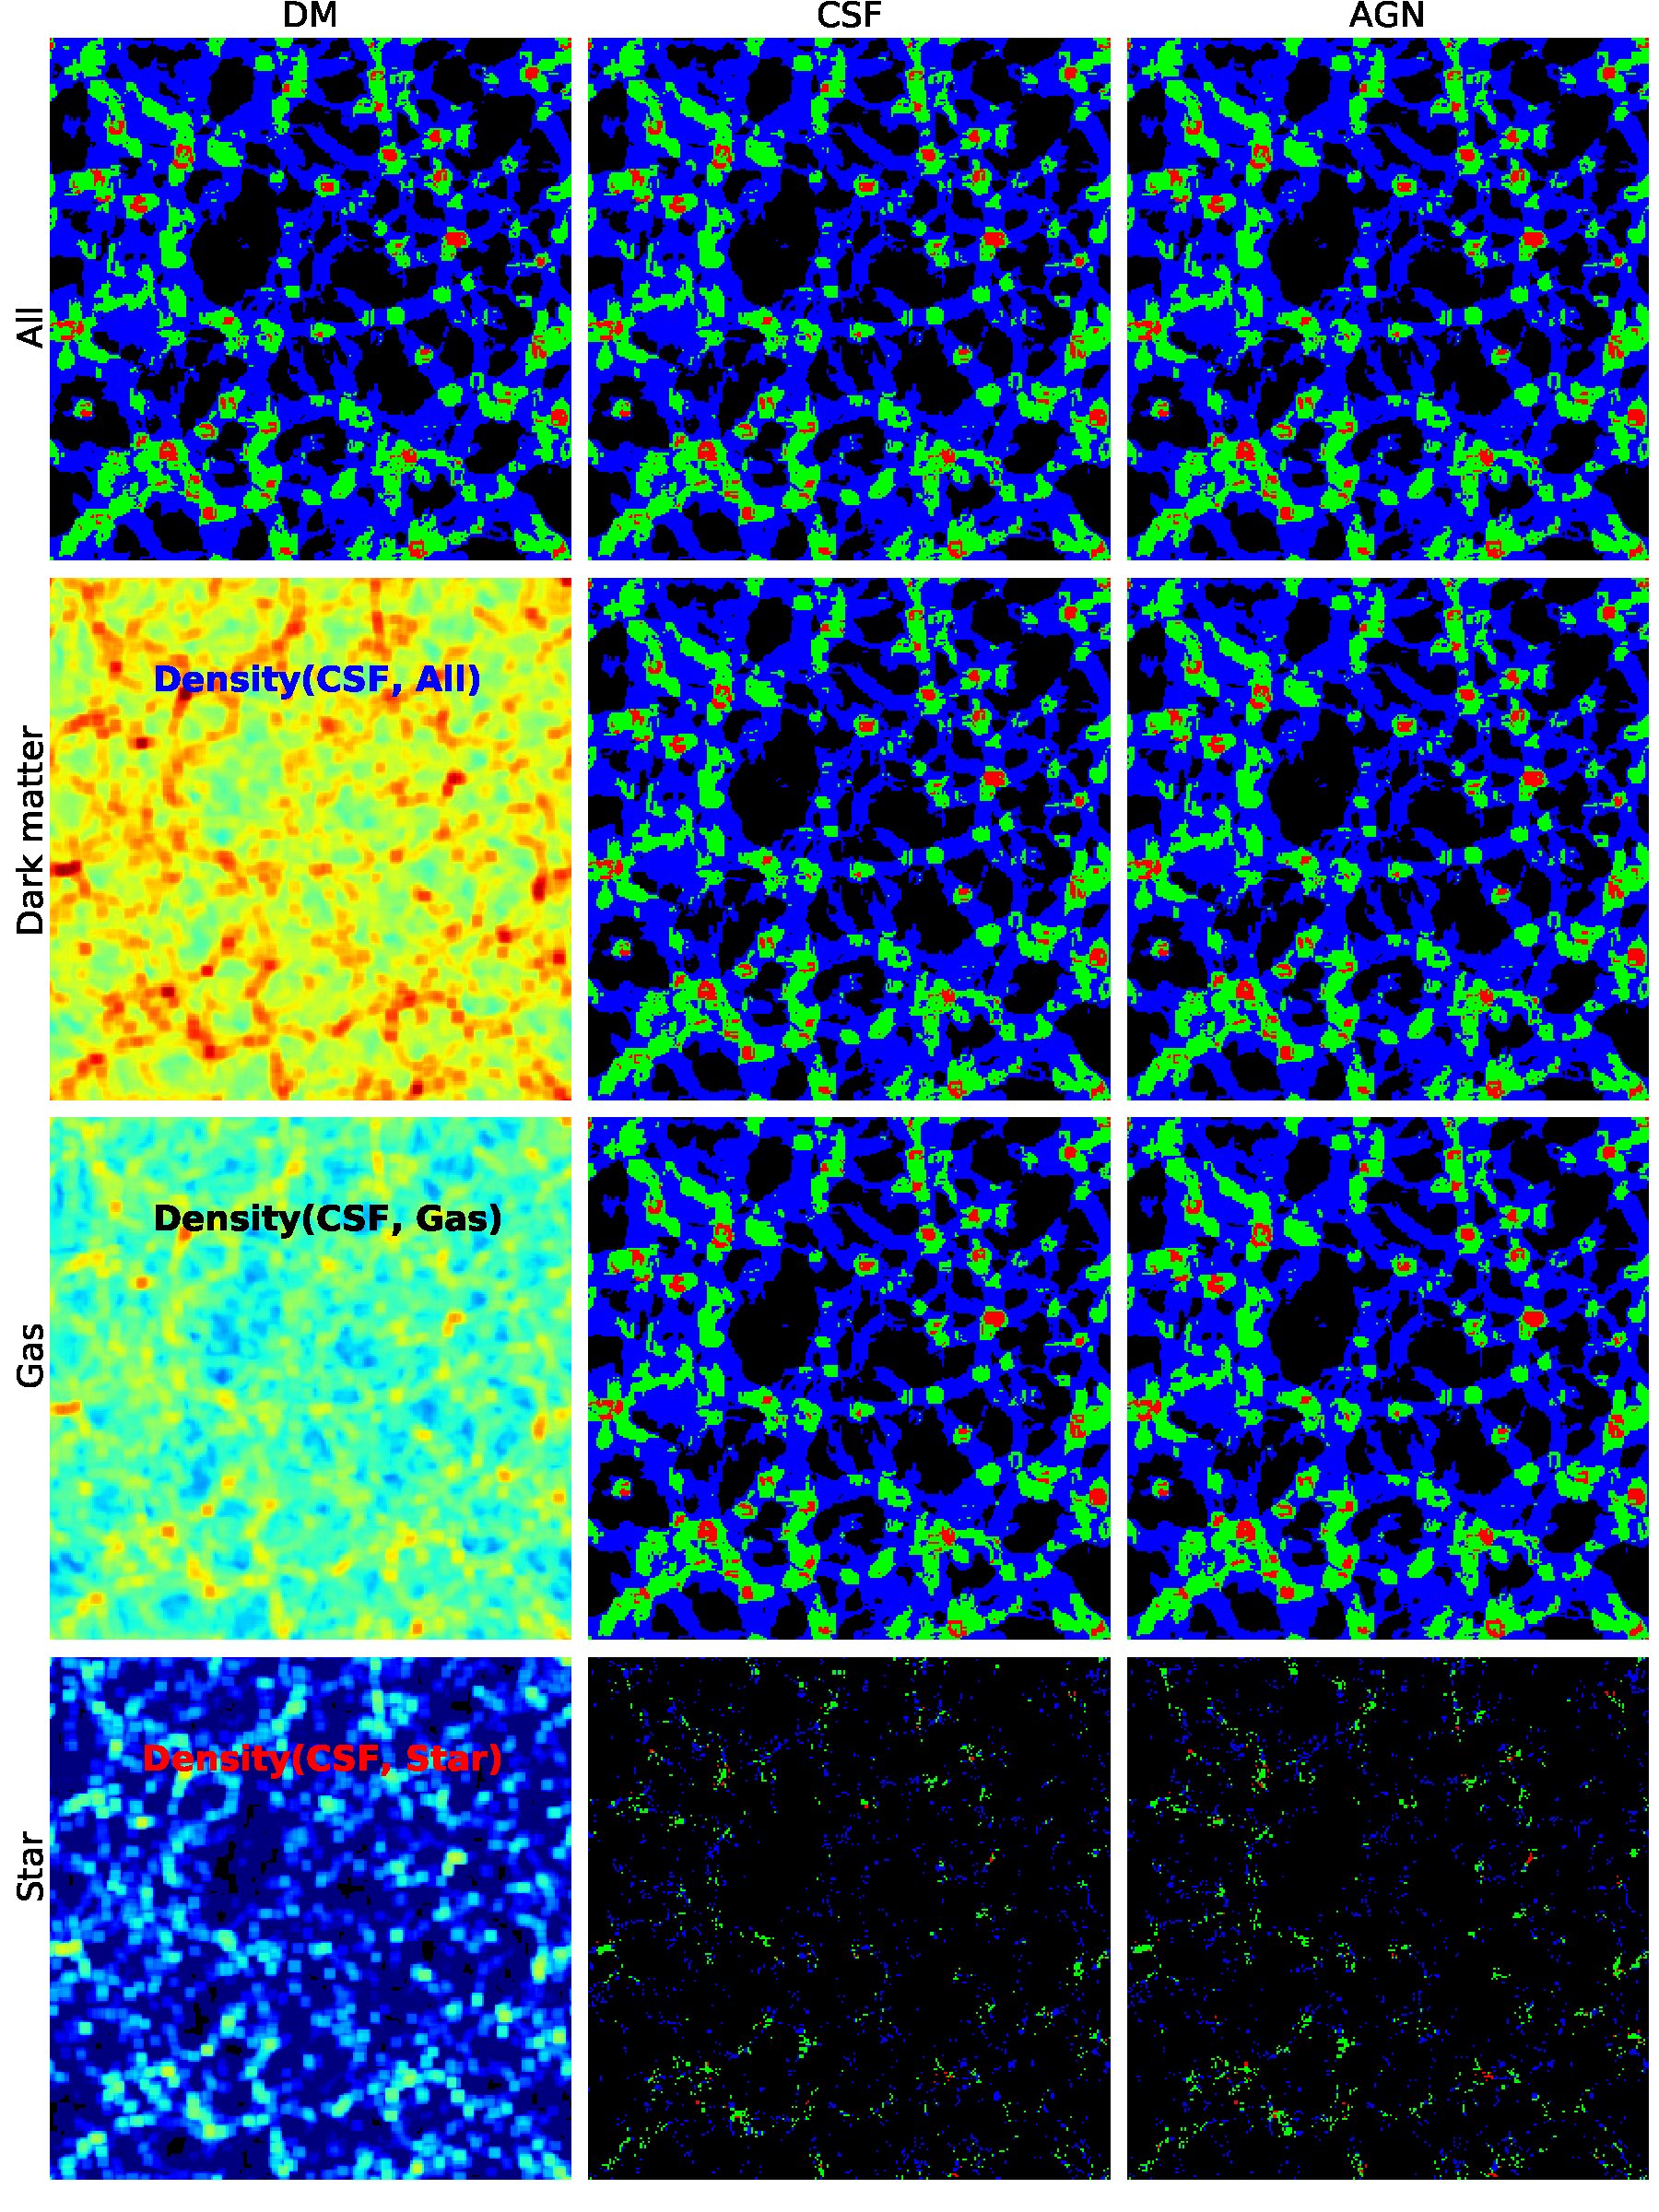
\includegraphics[width=0.5\linewidth]{image_show_V}
  \end{figure}
  \begin{textblock*}{3cm}(9.5cm,6cm)
    {Cui et al. 2018, Paper I, z=0, Vweb}
  \end{textblock*}
\end{frame}

\begin{frame}{The total mass fractions in different large-scale structures}
  \begin{figure}
    \includegraphics<1>[width=\linewidth]{Fractions-BE}
    \includegraphics<2>[width=\linewidth]{Fractions-gasweb}
    \caption{The mass and volume fractions of these \newline large-scale environments, Cui et al. 2018, Paper I}
  \end{figure}
\end{frame}

\begin{frame}
  \begin{textblock*}{8cm}(3cm,4cm)
    {\Huge Some preliminary results from Paper II}
  \end{textblock*}
\end{frame}

\begin{frame}{An illustration: the redshift evolution}
  \begin{figure}
    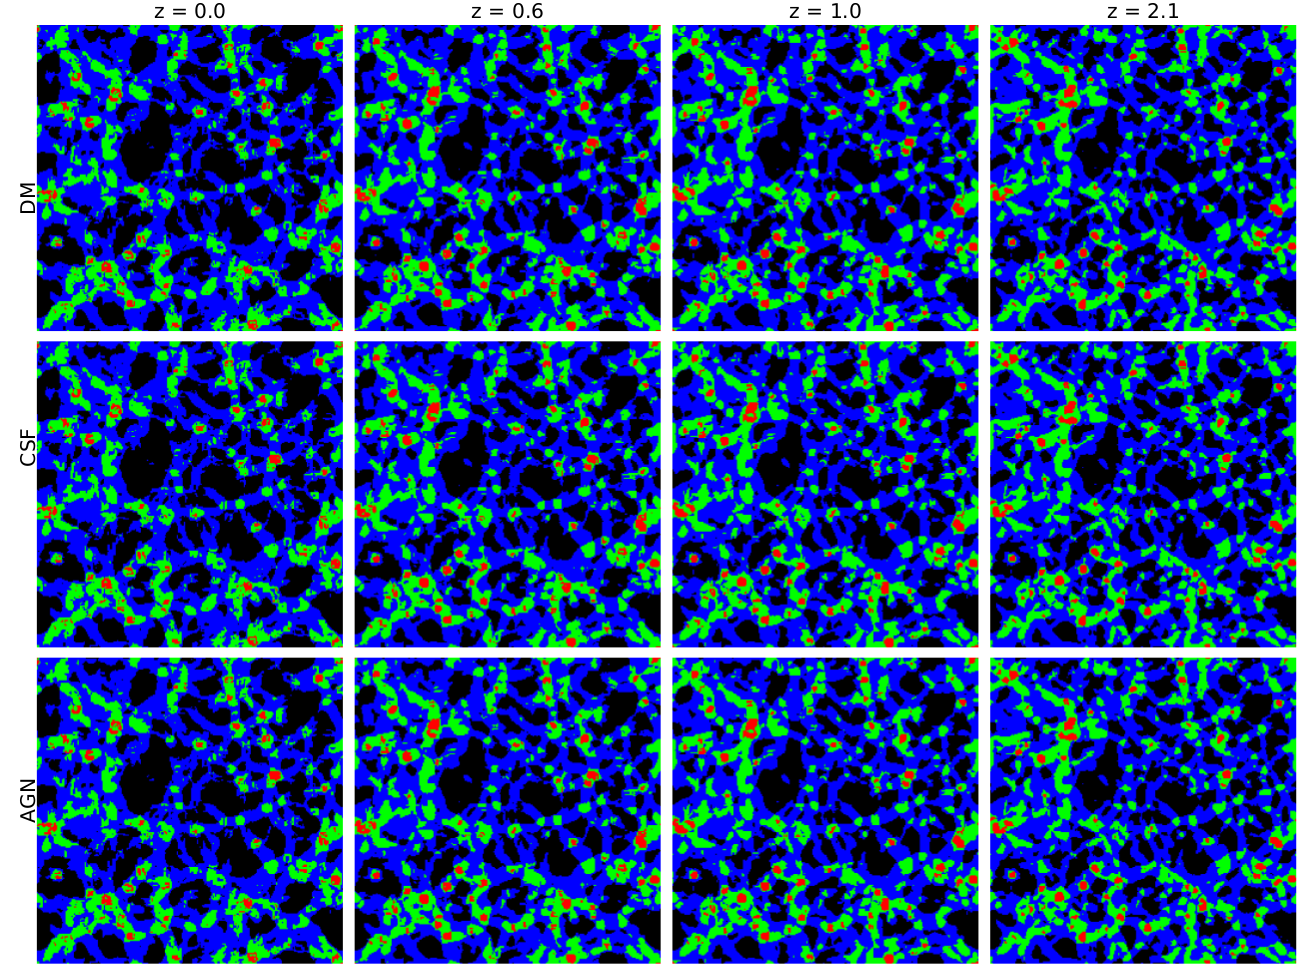
\includegraphics[width=0.8\linewidth]{Evolution-illustriation}
    \caption{large-scale environments classified by Vweb}
  \end{figure}
\end{frame}

\begin{frame}{The fraction evolution}
  \begin{figure}
    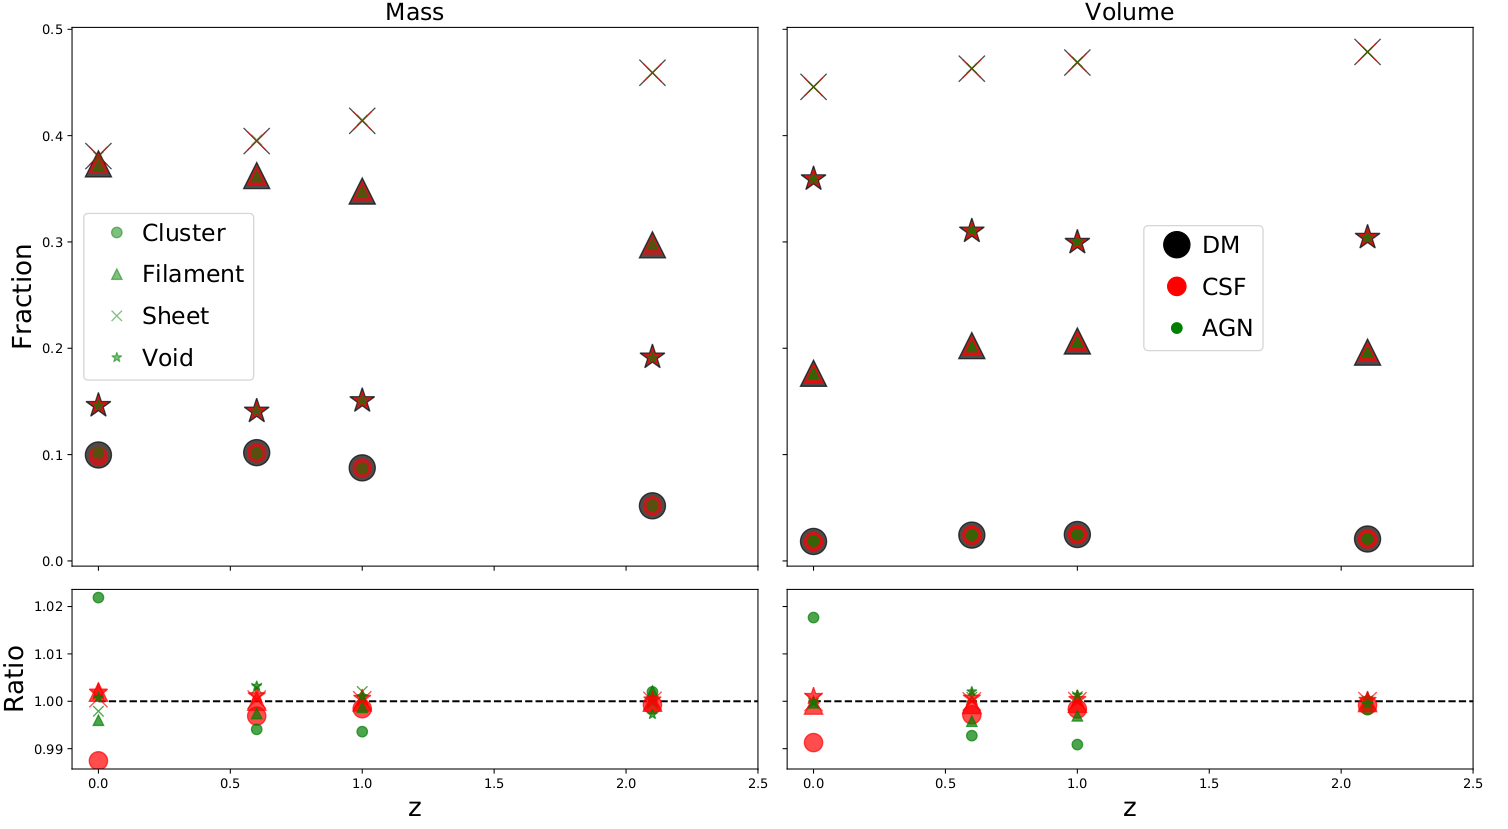
\includegraphics[width=0.9\linewidth]{Vweb-fraction-evolution.png}
    \caption{The mass (left) and volume (right) fractions evolution from the Vweb method. See Zhu \& Feng, 2017 for similar results.}
  \end{figure}
\end{frame}

\begin{frame}{The baryonic web}
  \begin{figure}
    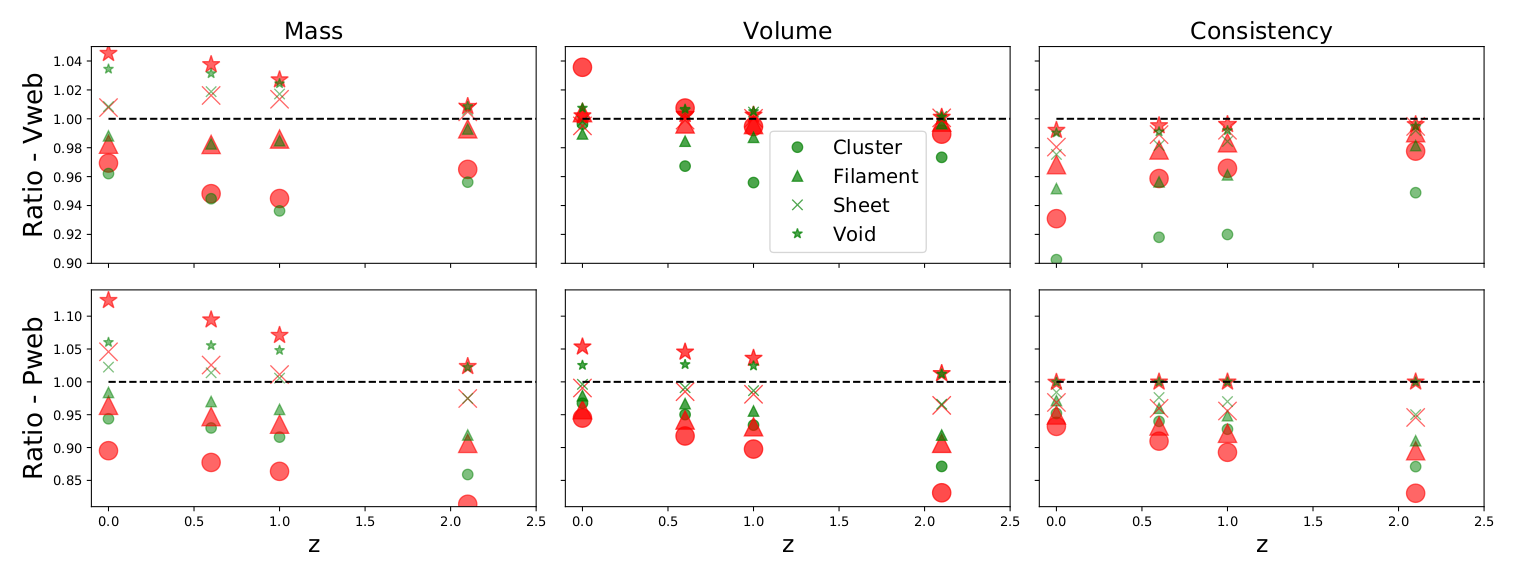
\includegraphics[width=\linewidth]{fraction-gasweb-evolution.png}
    \caption{The differences between the large-scale structures classified by gas and total matter.}
  \end{figure}
\end{frame}

\begin{frame}{The gas density-temperature diagram}
  \begin{figure}
    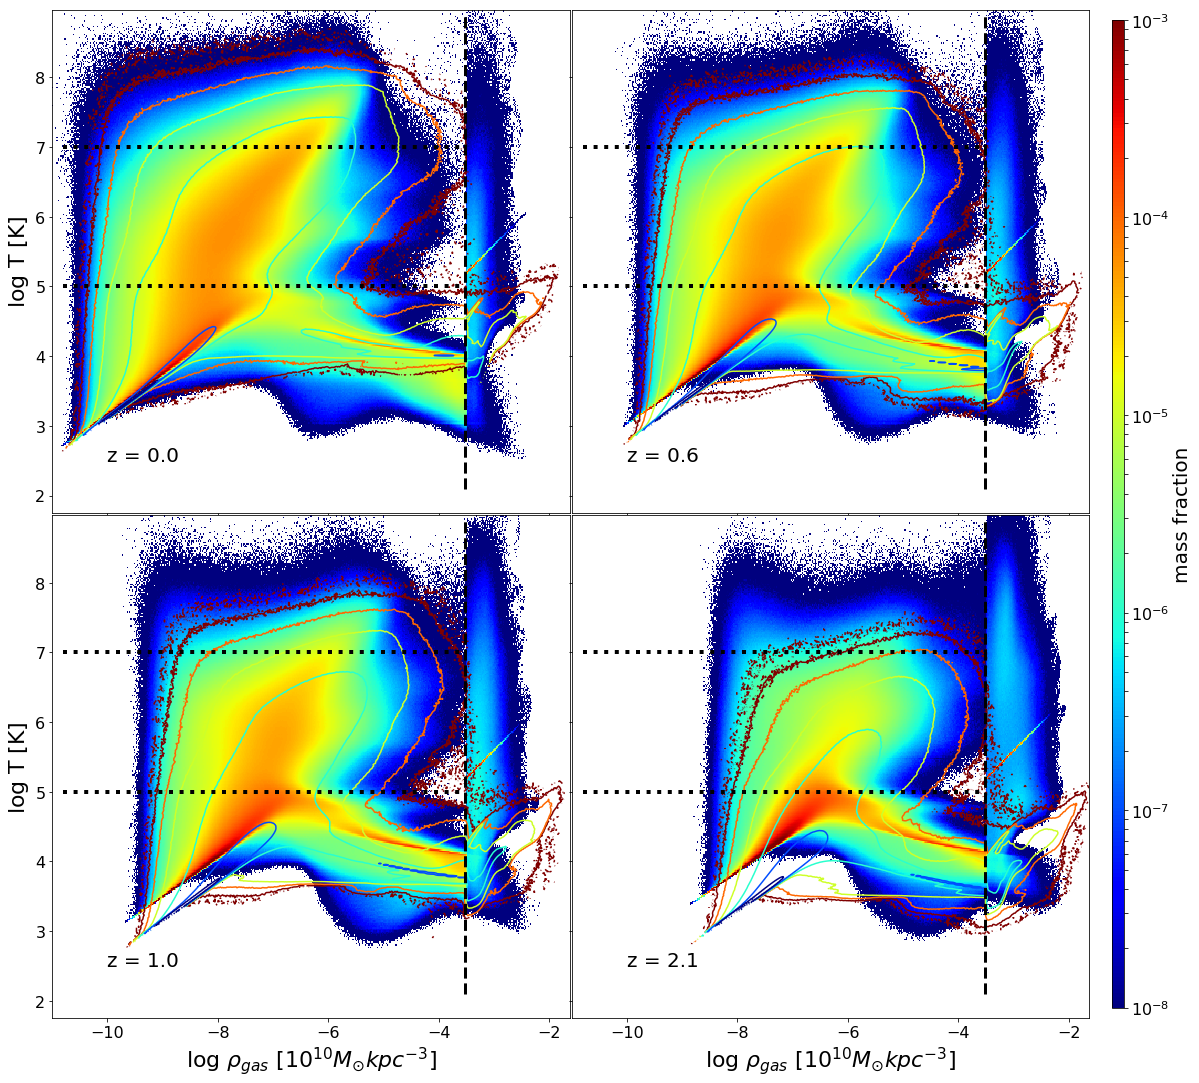
\includegraphics[width=0.7\linewidth]{RT-evolution.png}
  \end{figure}
\end{frame}

\begin{frame}{The gas density-temperature diagram in different large-scale environments}
  \begin{figure}
    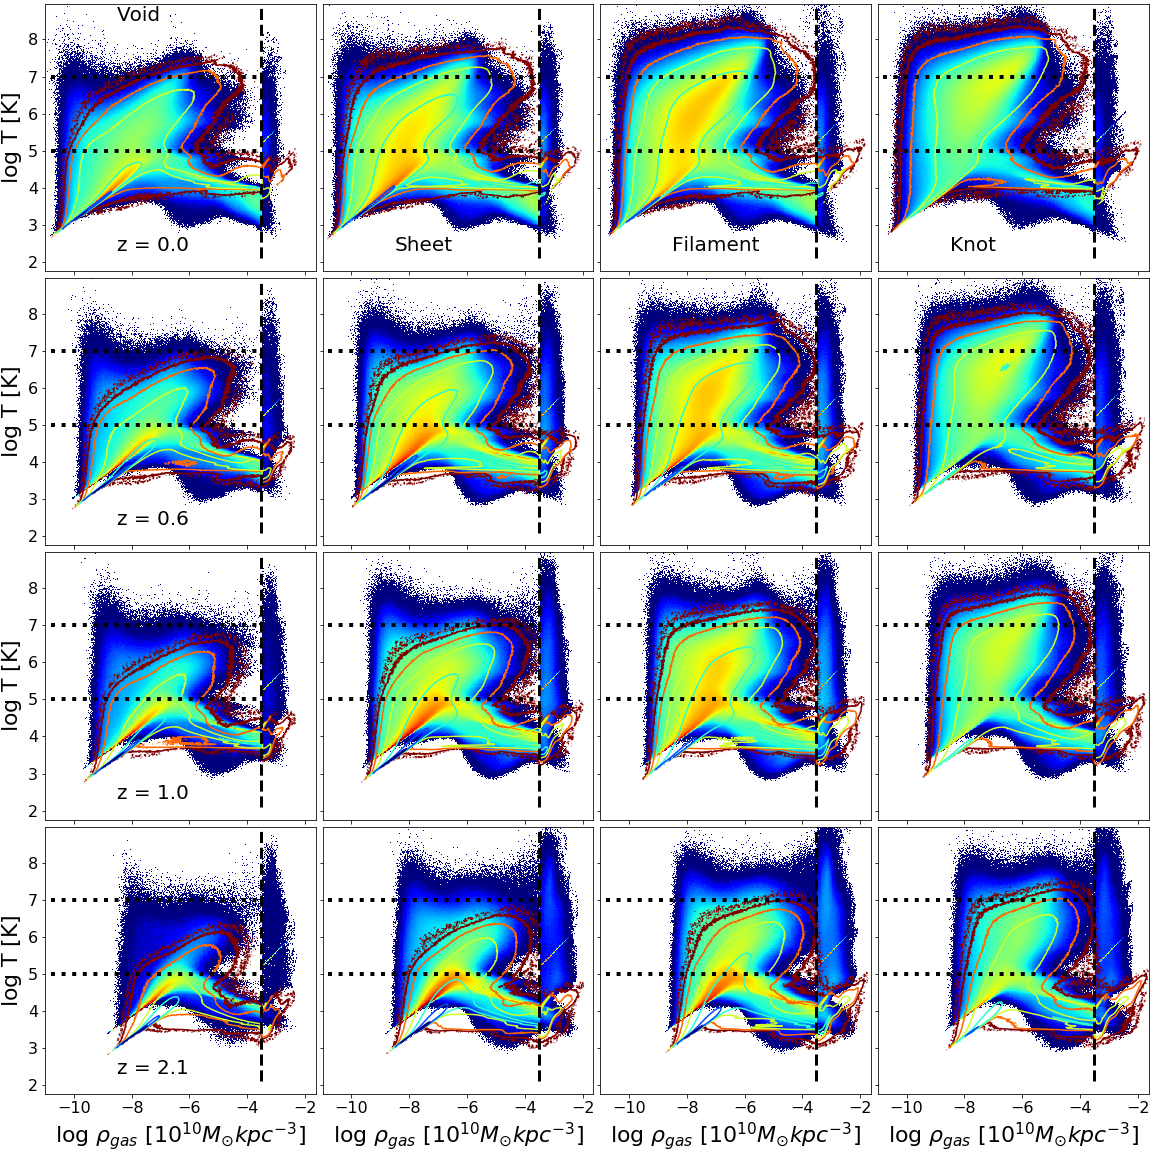
\includegraphics[width=0.6\linewidth]{RTE-evolution.png}
  \end{figure}
\end{frame}

\begin{frame}{The fractions in different gas components.}
\begin{table}
\fontsize{10}{10}\selectfont
\caption{The distribution of different baryon components in different environments. The AGN results are the first value with the CSF results follow in the bracket.}
  \begin{tabular}{c|c|c|c|c}
       & Voids & Sheets & Filaments & Knots \\
       \hline
       & & z = 0 & & \\
       \hline
    $f_{M, gas}$ & 0.15 (0.16) & 0.38 (0.39) & 0.37 (0.36) & 0.1 (0.09) \\
    $f_{M, star}$ & 0.08 (0.06) & 0.33 (0.29) & 0.44 (0.48) & 0.15 (0.17) \\
    $f_{M, hot gas}$ & 0.002 (0.003) & 0.04 (0.05) & 0.46 (0.50) & 0.49 (0.45) \\
    $f_{M, WHIM}$ & 0.05 (0.06) & 0.30 (0.31) & \alert{0.51 (0.50)} & 0.14 (0.13) \\
    \hline
       & & z = 0.6 & & \\
       \hline
    $f_{M, gas}$ & 0.14 (0.14) & 0.39 (0.39) & 0.37 (0.36) & 0.11 (0.11) \\
    $f_{M, star}$ & 0.05 (0.03) & 0.28 (0.22) & 0.47 (0.48) & 0.21 (0.27) \\
    $f_{M, hot gas}$ & 0.001 (0.000) & 0.01 (0.003) & 0.23 (0.15) & 0.76 (0.85) \\
    $f_{M, WHIM}$ & 0.03 (0.03) & 0.25 (0.23) & \alert{0.53 (0.52)} & 0.20 (0.22) \\ 
    % \hline
    %   & & z = 1.0 & & \\
    % $f_{M, gas}$ & 0.14 (0.14) & 0.40 (0.40) & 0.36 (0.35) & 0.10 (0.10) \\
    % $f_{M, star}$ & 0.03 (0.02) & 0.26 (0.20) & 0.48 (0.48) & 0.22 (0.29) \\
    % $f_{M, hot gas}$ & 
    % $f_{M, WHIM}$ &    
    % \hline
    %   & & z = 2.1 & & \\
    % $f_{M, gas}$ &  0.18 (0.18) & 0.45 (0.45) & 0.31 (0.31) & 0.06 (0.06) \\
    % $f_{M, star}$ & 0.02 (0.02) & 0.23 (0.20) & 0.52 (0.50) & 0.24 (0.28) \\
    % $f_{M, hot gas}$ & 
    % $f_{M, WHIM}$ &    
  \end{tabular}
\end{table}
\end{frame}

\section{conclusion and future prospects}
\begin{frame}
  \frametitle{Conclusion}
  {\Large
  \begin{itemize}
    \item The baryon models have a weak impact on the matter distributions at large scale.
    \item Gas is a unbiased tracer of dark matter for these large-scale structures, especially filament.
    \item Although the whole gas is almost equally assigned into sheet and filaments, the most WHIM is located in the filament structures while the hot gas is basically located in filaments and knots.
  \end{itemize}}
\end{frame}

\begin{frame}
  \frametitle{Future prospects}
  Connecting hydrodynamical simulations with observations through mock images.
  \begin{itemize}
    \item Optical: pymgal
    \item Xray: pymxc 
    
        spectrum is coming from Xspec library, interpolated with gas properties from hydrosimulations to produce the SIMPUT format, this file will use SIXTE (a monte-carlo simulation toolkit for the Athen XIFU) to produce the eventlist.
    \item SZ: pymsz
    \item Radio: pymr
  \end{itemize}

  \only<2>{
  My personal interests to HUBS:
  \begin{itemize}
    \item[1] theoretical analysis pipeline with pymxc.
    \item[2] Using HUBS to constrain cosmology models/parameters.
  \end{itemize}}
\end{frame}

% \begin{frame}{ ~ }
%     {\Huge Thank you.}
% \end{frame}

\end{document}
